\ylDisplay{Konfokaalne mikroskoop} % Ülesande nimi
{Mihkel Rähn} % Autor
{lõppvoor} % Voor
{2009} % Aasta
{G 7} % Ülesande nr.
{4} % Raskustase
{
% Teema: Geomeetriline-optika
\ifStatement
Harilikest mikroskoopidest parema ruumilise lahutuse saamiseks kasutatakse konfokaalseid
mikroskoope. Juuresoleval joonisel on kujutatud konfokaalse mikroskoobi põhielemendid:
objektiiv, läätsed L$_1$ ja L$_2$ ning nende ühises fokaaltasandis asuv väike ringikujuline ava.
Joonisel on samuti esitatud optilisel peateljel asuvast väikesest uuritavast esemest lähtuvate
kiirte käik.
Objektiivi fokaaltasandist kaugemal ja lähemal olevatest
objektidest lähtuvad kiired ei läbi enamuses ava, vaid neelduvad ava servadel.
Kõrvalnähtusena vaateväli kitseneb. Kui kaugel optilisest peateljest
võib olla objektiivi fokaaltasandis olev ese, et see oleks veel nähtav? Läätsede L$_1$, L$_2$ ja objektiivi fookuskaugused on vastavalt $f_1$, $f_2$ ja $f_{\mathrm{obj}}$, ava läbimõõt $d$.

\begin{center}
	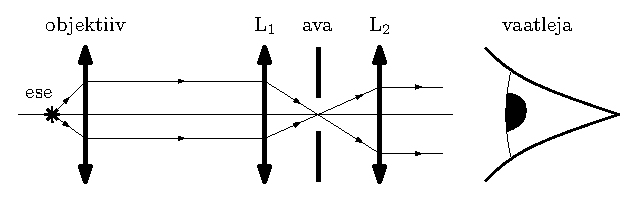
\includegraphics[width=0.8\linewidth]{2009-v3g-07-G_konfokaalne_mikroskoop.eps}
\end{center}
\fi


\ifHint
Piisab kahe ettevaatlikult valitud kiirte käikude vaatlemisest.
\fi


\ifSolution
Lahenduse optiline skeem on toodud joonisel. Konstrueerimisel tuleb
läätsede vahelised kiired joonestada paralleelsed ja läätsede keskpunkte läbivad.
Sellisel juhul annavad need kiired eseme ja ava tasandil vastavalt eseme ja kujutise
asukohad.

\begin{center}
	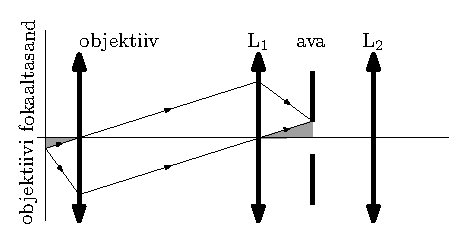
\includegraphics[width=0.8\linewidth]{2009-v3g-07-G_konfokaalne_mikroskoop_lah.eps}
\end{center}

Värvitud kolmnurgad on NNN tunnuse järgi sarnased. Seetõttu kehtib võrdus
\[
\frac{d}{2f_1}=\frac{r_{\mathrm{ese}}}{f_{\mathrm{obj}}},
\]
millest
\[
r_{\mathrm{ese}}=\frac{d\cdot f_{\mathrm{obj}}}{2f_1}.
\]
\fi
}